\documentclass[12pt,twocolumn]{article} %TWO COLUMNS
\usepackage{graphicx}
\usepackage{wrapfig}
\usepackage[hidelinks]{hyperref}
\usepackage{booktabs}
\usepackage{titling} 
\usepackage{abstract}
\usepackage{titlesec}
\usepackage{enumerate}
\bibliographystyle{vancouver}
\usepackage[hmarginratio=1:1,top=15mm,left=15mm,columnsep=15pt]{geometry}% MARGINS
\usepackage[small,labelfont=bf,up,textfont=it,up]{caption} %CAPTIONS FORMAT
%SECTIONS AND SUBSECTIONS
\renewcommand\thesection{\Roman{section}} 
\renewcommand\thesubsection{\roman{subsection}} 
\titleformat{\section}[block]{\large\scshape\centering}{\thesection.}{1em}{} 
\titleformat{\subsection}[block]{\large}{\thesubsection.}{1em}{} 
\titlespacing*{\section}
{0pt}{\baselineskip}{\baselineskip}
% TITLE AND ABSTRACT
\renewcommand{\abstractnamefont}{\normalfont\bfseries}
\renewcommand{\abstracttextfont}{\normalfont\small\itshape}
\pretitle{\begin{center}\Huge\bfseries} 
	\posttitle{\end{center}} 
\title{Problems that arise when peforming a small-scale soil microbiome analysis and how to prevent them} 
\author{\normalsize University College London \\}
\date{\today}
\renewcommand{\maketitlehookd}{
	\begin{abstract}
		\noindent
	 	Microbiome analysis is an area of research that is currently experiencing a major growth, with over 10000 articles published on the topic in the last 5 years. A severe decrease in price of both the DNA sequencing and computational power in the recent years, led to this data-driven area of research becoming more accessible. In order to determine whether it is possible to generate valid results from a small-scale analysis, 30 samples of soil were collected in Central London and High-Performance Computing clusters were used together with software for mictobiome analysis to assess the uniformity of the samples and discover correlations between the chemical and biological content. This paper focuses on three main aspects - assessing the validity of the data for further use by other researchers, investigating the relationships between the samples and analysis of the issues that hamper the research on such a small dataset.
	 \end{abstract}
}
%INDENTS
\setlength{\parindent}{5mm}
\setlength{\parskip}{0mm}
\setlength{\intextsep}{3mm}
\setlength{\textfloatsep}{5mm}
% DOCUMENT
\begin{document}
	
\maketitle
% IMPROVE THE INTRODUCTION
%
%

\section{Introduction}
The area of microbial ecology is a comparatively recent discipline -  majority of articles on this topic were published in the period of 2013-2017. A multitude of reasons led to such as growth in the area with the biggest one being the constant decrease of price of sequencing techniques, which allows to analyse the genetic composition of soil directly and study the interactions between bacteria that are hard to cultivate \textit{in vitro}.
\par
One of the main areas of development in the field of microbiome analysis is the creation of big databases with a variety of samples from a range of biomes. The most successful project in this area is the EMP - Earth Microbiome Project\cite{Gilbert2014}. It was started in 2010 and focuses on developing a global catalogue of Earth's microbial diversity, which can be used not only to perform studies on large datasets in order to find correlations within them, but also as a point of reference for specialists in other areas looking for insight into the microbial ecology of different locations and environments. The samples that were collected during our research could potentially be included in the EMP however, the assessment of validity of the genetic sequences extracted should be performed.
\par
The research described in this paper was focused on performing such task, as well as investigating whether a small-scale microbiome analysis, in general, can provide valid scientific results. The low number of samples (30) that were collected during this experiment, the low diversity of conditions they were collected in, coupled with an inadequate quality of some kits used for analysis created an array of problems, which are going to be described in this paper, along with the methods.
\par
Our method was based on extracting the 16S DNA from the prokaryotes in the samples collected, using a variety of kits. Since soil is known to have a very high concentration and diversity of bacteria\cite{Nannipieri2003,Torsvik1996}, such methods produce large amounts of data, which had to be analysed using specialised software.
% METHODS
%
\section{Methods}
The analysis was performed on 30 samples of soil collected in Central London in October 2017.  Metadata, such as moisture, temperature, footfall was collected on the spot, while other aspects such as pH and concentrations of various ions was measured in the laboratory using the \textit{HI3895 Soil Testing Kit}. Then 4 different kits were used in a workflow designed to extract the sequences of 16S DNA from the prokaryotes in the soil, following the instructions provided by manufacturer of each kit.
\par
First, DNA was extracted using the \textit{DNeasy PowerSoil Kit} and PCR primers were designed that contained Golay barcodes, allowing multiple samples to be sequenced simultaneously. \textit{BioMic PCR Kit} was used with the primers to perform the PCR. The solution acquired as the result of PCR was purified using \textit{QIAquick PCR Purification Kit} and then the concentration of dsDNA was measured using \textit{SpectraMax Quant AccuClear Nano dsDNA Assay Kit}. Using the information on DNA concentration all of the samples were subsequently diluted to equal concentrations and sequencing was done on \textit{Illumina's MiSeq} sequencer. Quality control was performed throughout this stage of the experiment. This workflow returned the DNA sequences that were used for downstream \textit{in silico} analysis.
\par
\textit{In silico} stages of the research were performed using the QIIME\footnote{Version 1.9.1} package\cite{Caporaso2010,Kuczynski2012}, which allows users to do high-throughput sequence analysis. Parts of analysis that required severe computational power were performed on the Cirrus High-Performance Computing system. QIIME package has a basic pipeline that was used to transform the raw data into the form that can be used for statistical analysis, which is described below.
\par
The first step is validation of the initial data, such as mapping and fasta files, followed by read joining, which joins the forward and reverse fasta files. After that, sequences are grouped back into 30 groups that represent the 30 samples. This stage is commonly called demultiplexing, and involves removal of the barcodes that were introduced in the PCR stage. After the demultiplexed fasta file is produced, OTU (Operational Taxonomic Unit) are picked. OTU picking groups closely related sequences (97\% similarity in our case, which corresponds to species-level sequence identity\cite{STACKEBRANDT1994}) into operational units, which are then used for further analysis.
\par 
OTU picking requires a referencing database. In this research, SILVA\footnote{Release 132, April 10, 2018}\cite{Quast2012} database was used, which is more up-to-date than Greengenes\cite{McDonald2012} database provided with QIIME. OTU picking and demultiplexing are generally the most expensive stages, in terms of computational power. For this reason they were performed on the Cirrus HPC and most of the downstream analysis was performed on a local machine. 
\par
QIIME package provides a variety of scripts designed to analyse the genetic sequences data. However, it should be noted that while providing users with variety of methods to perform the analysis, the figures created by the scripts provided are subpar. This lead to a collection of scripts that were used to perform some of the analysis and construct the figures, which can be found on the dedicated GitHub repository\cite{Anonymous2018}. The repository also features additional results that are out of scope of this paper. The scripts were created using various python packages, such as numpy, scipy, pandas, seaborn and matplotlib, which greatly aid in data visualisation and statistical calculations.
\par
A method that is useful to determine whether the samples we collected are representative of the biome is provided in the Sourcetracker package\cite{Knights2011}. This collection of scripts allows users to track proportion of each \textit{source} in each \textit{sink}, in our case \textit{source} and \textit{sink} being different samples of soil from Release 1 of the EMP and our samples respectively. Sourcetracker package is available with QIIME however, Sourcetracker2 has been developed recently, which was used due to being more accurate and functional. 
The Sourcetracker workflow produces a matrix that displays how much of each source is present in each of our samples.
\par
In an attempt to find a correlation between metadata and the diversity of our samples, scripts included in the QIIME package were used and metadata was transformed into numeric form, with results from \textit{HI3895 Soil testing Kit} treated as values on exponential scale. Analysis was performed using ANOSIM\cite{CLARKE1993}, PERMANOVA\cite{Tang2016} and a collection of other statistical methods, which calculate the correlation between the distance matrix and pH, potassium, nitrogen and phosphorus content.
\par
Furthermore, to assess the taxonomic composition of our samples a taxonomic assignment using the SILVA\cite{Quast2012} database was done. The classical microbiotic analysis was performed as well, that investigates the diversity of the samples.
%
% RESULTS
%
\section{Results} 
During the OTU picking stage, over 4.5 million sequences were recovered from raw data, with 16448 of them being unique. However, it should be noted, that due to use of closed-reference OTU picking, almost 800 thousand sequences (17\%) were removed from the downstream analysis because no match was found in the database. 
\begin{figure}[ht!] %alpha diversity
	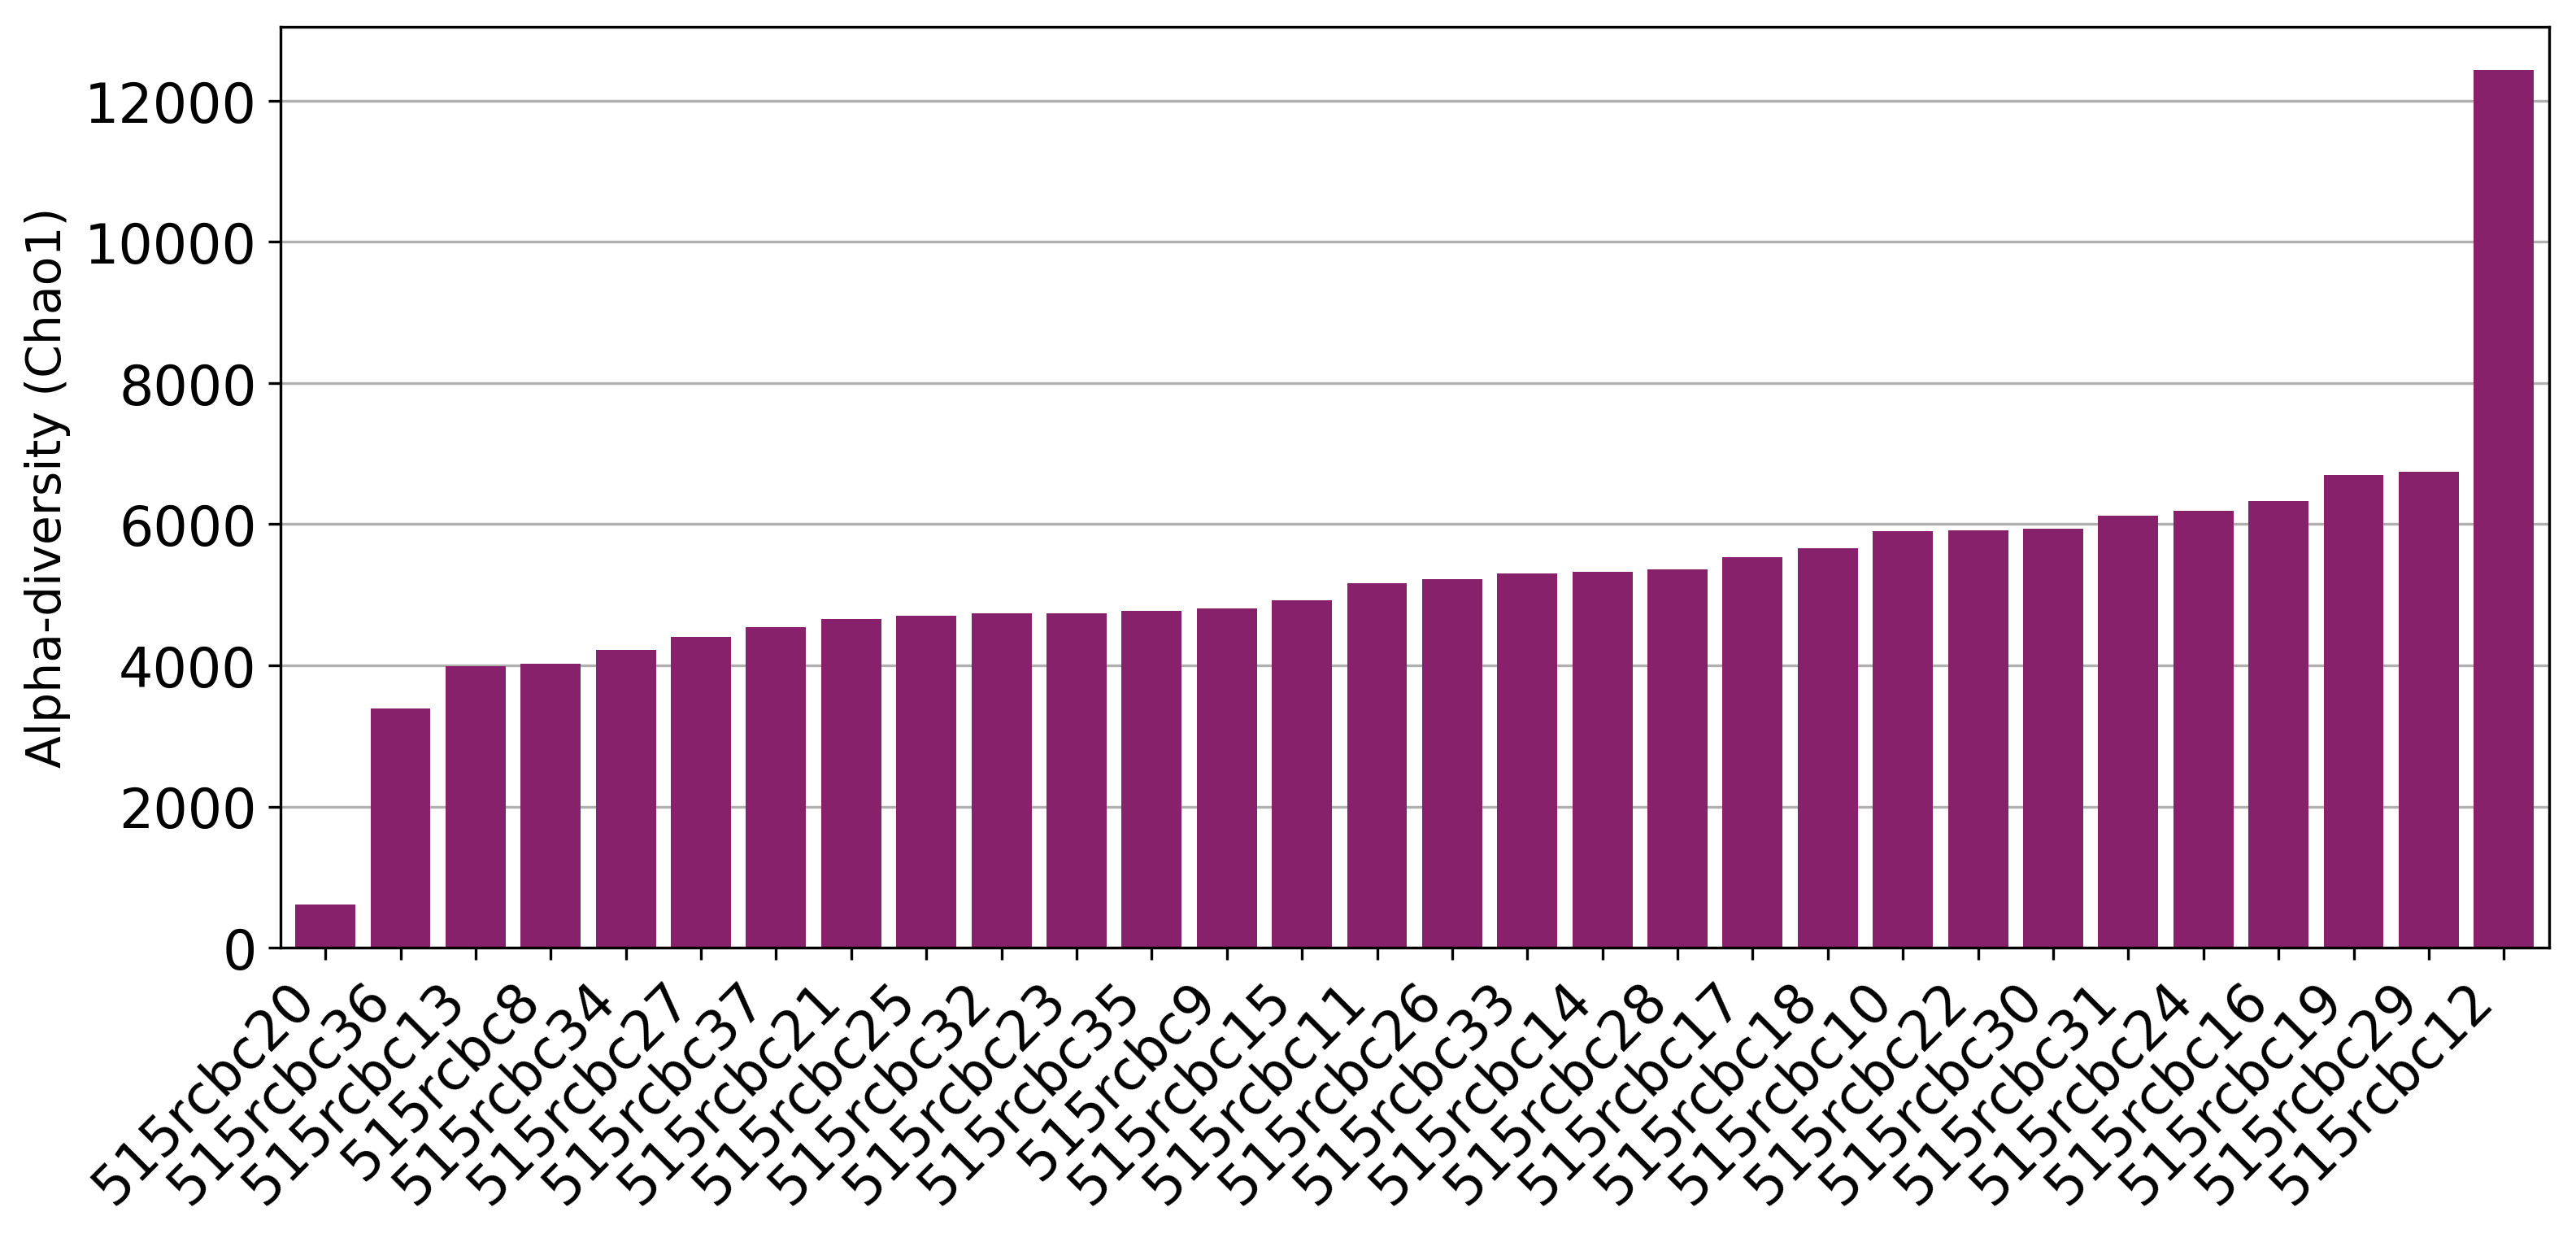
\includegraphics[width=\linewidth]{chao1_alpha.png}
	\caption{Alpha diversity (Chao1) for each of 30 samples.}
	\label{fig:alpha_diversity}
\end{figure}
\par
Using the OTU table that was produced as a result of the OTU picking, alpha diversity was measured, which assesses the number of unique OTU for each sample. The distribution of alpha diversities between the samples is presented in Figure \ref{fig:alpha_diversity}. As we can see from the Figure, most samples have similar values for alpha diversity, with a mean of 5188. Samples \textit{515rcbc12} and \textit{515rcbc20} are the outliers with alpha diversity of 608 and 12429 respectively. If the 2 outliers are removed, the standard deviation for the dataset is 843, which shows that the samples are tightly grouped.
\begin{figure}[ht!] %beta diversity
	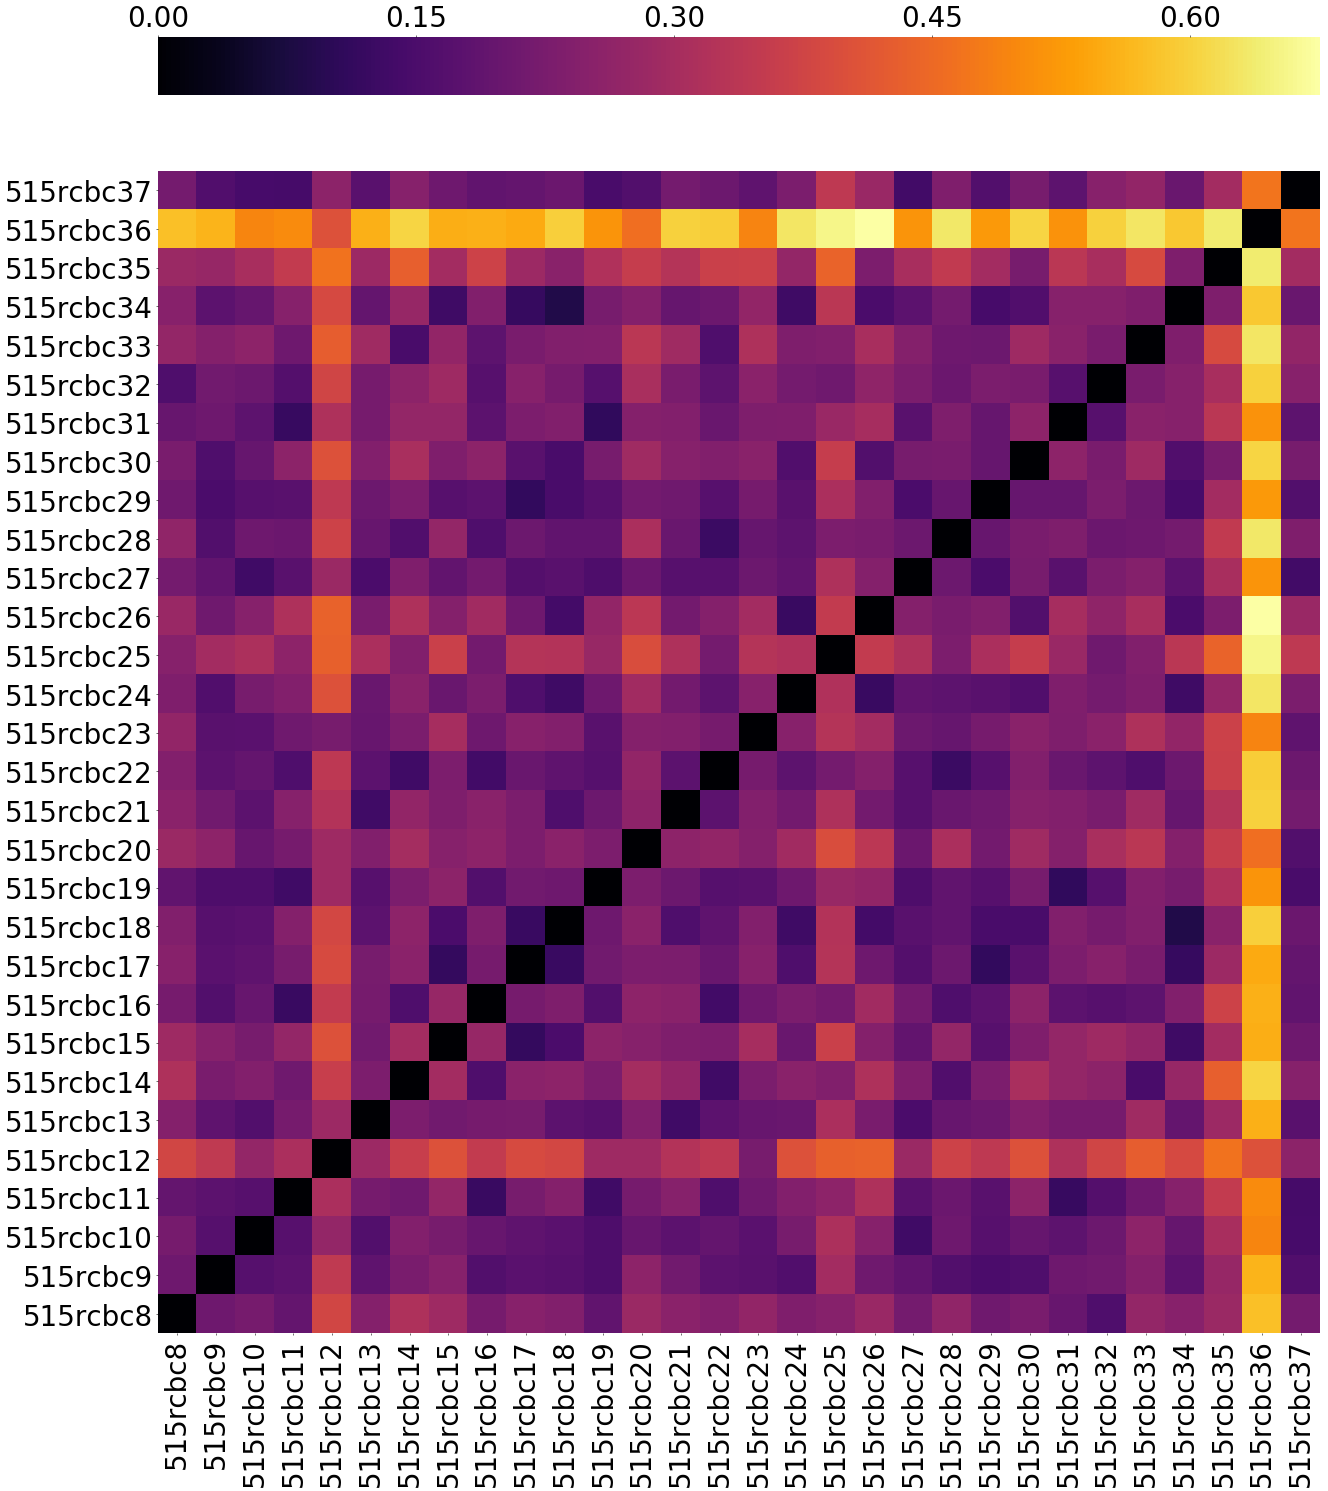
\includegraphics[width=\linewidth]{unweighted_beta.png}
	\caption{Beta diversity (unweighted unifrac) matrix, presented as a heat map.}
	\label{fig:beta_diversity}
\end{figure}
\par
In order to further investigate the uniformity and clustering of the samples, beta-diversity analysis was performed. The heat map presented in Figure \ref{fig:beta_diversity} is a graphical representation of beta-diversity between the samples, with higher values representing higher divergence.
\par
Sample \textit{515rcbc36} can be identified as the most divergent from the rest, with \textit{515rcbc12} being an outlier as well. The mean beta-diversity without sample \textit{515rcbc36} is 0.237, with standard deviation of 0.066, further supporting the hypothesis of the uniformity of the samples.
\par
In order to determine whether the data obtained in a small-scale microbiome analysis is sufficient to find correlations within the dataset several statistical analyses were performed. First, statistical method of ecology analysis ANOSIM\cite{CLARKE1993} was used together with the collected metadata and distance matrices to find any correlations, results are presented in Table 1.
\begin{table}[ht!] %statistical table
	\begin{center}
		\label{tab:table_correlation}
		\begin{tabular}{c|c|c}
			\textbf{Category} & \textbf{R-value} & \textbf{p-value}\\
			\hline
			pH & -0.109 & 0.869\\
			Potassium & 0.224 & 0.023\\
			Nitrogen & 0.120 & 0.120 \\
			Phosphorus & 0.201 & 0.058\\
		\end{tabular}
		\caption{Correlation between metadata and beta-diversity, calculated using ANOSIM\cite{CLARKE1993} method, with external data treated as values on exponential scale.}
	\end{center}
\end{table}
\par
Since the R-value is close to 0 for all four parameters, it can be safely assumed that there is no statistically significant correlation between the chemical properties and the diversity in our samples. Other methods of statistical analysis, such as PERMANOVA\cite{Tang2016} confirmed this assumption because attempts to find non-linear correlations were also unsuccessful.
\par
The assessment of taxonomic composition of the samples was performed as well, with the taxonomic referencing database included in the SILVA database used to assign taxonomy to most of the OTUs. Figure \ref{fig:top_taxa} highlights the top 10 most abundant phyla across all of the samples. These 10 phyla represent 96\% of the sequences. More detailed plots on the topic of taxonomy are also available on GitHub\cite{Anonymous2018}.
\begin{figure}[ht!] %top phyla
	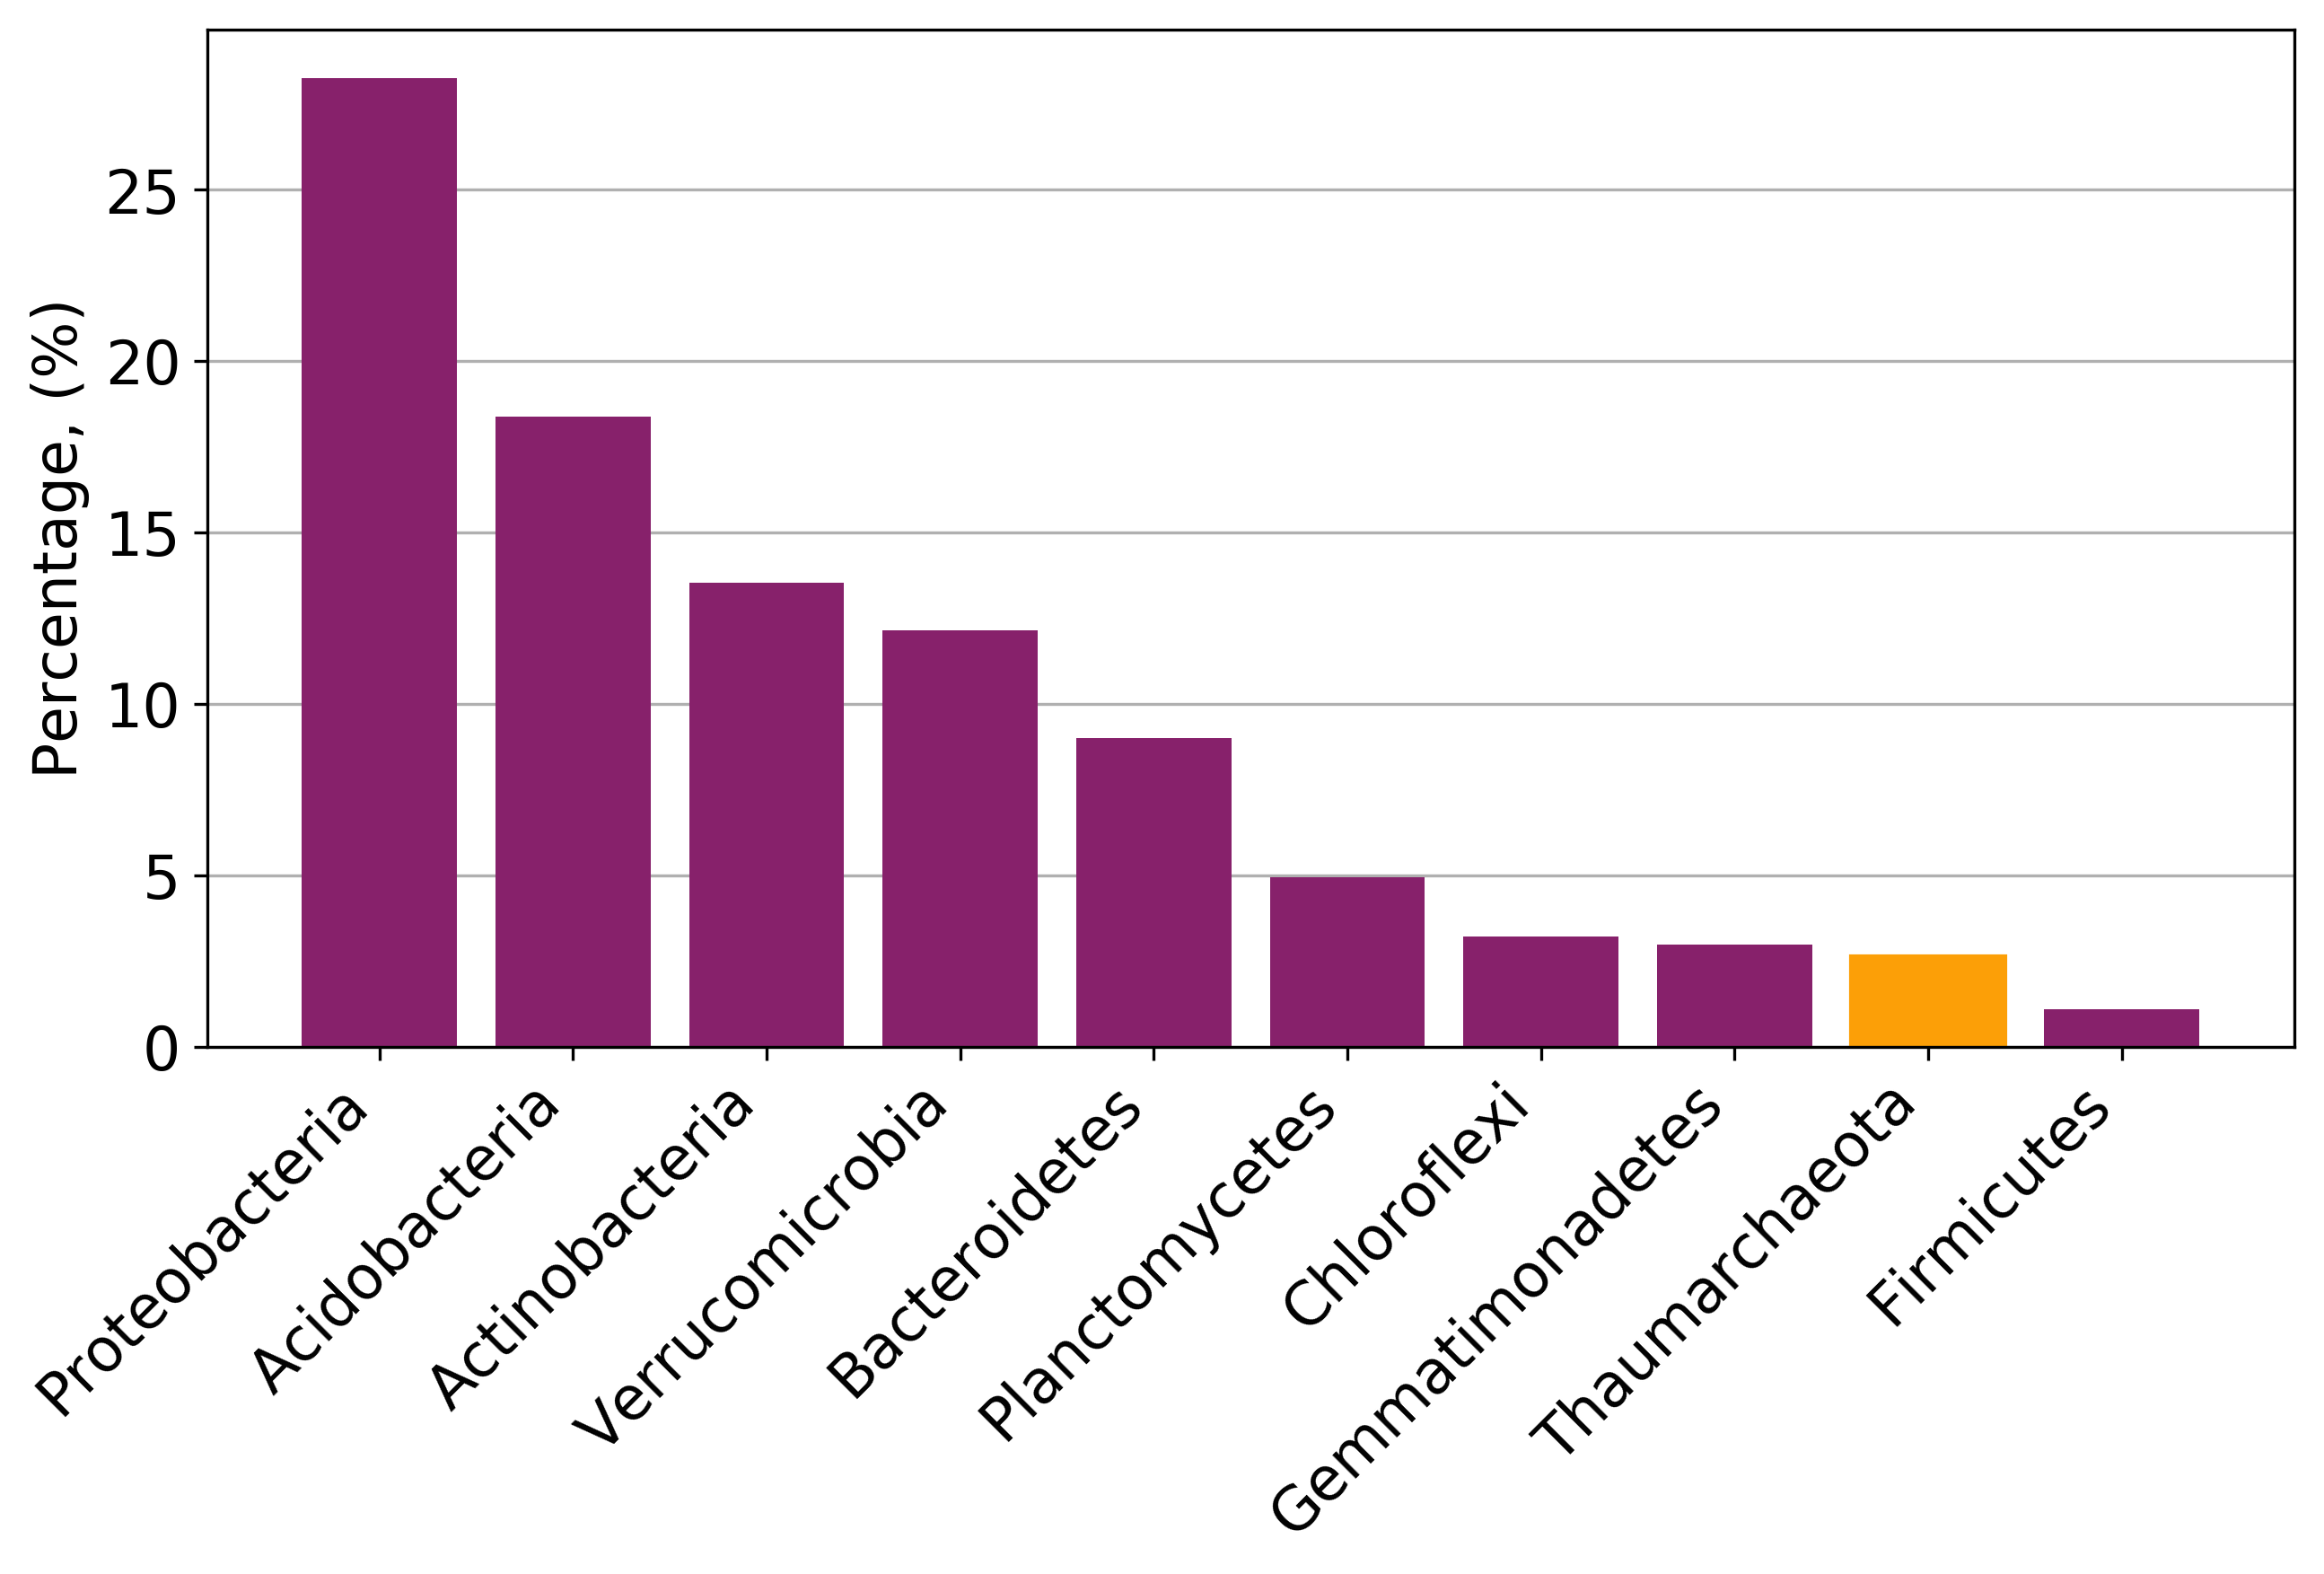
\includegraphics[width=\linewidth]{top_10.png}
	\caption{Proportion of most popular phyla in samples. The orange bar represents the only phylum from the Archea domain. These 10 phyla represent 96\% of species in our samples.}
	\label{fig:top_taxa}
\end{figure}
\par
The only phylum from the \textit{Archea} domain is \textit{Thaumarchaeota} and the rest of the sequences have a bacterial origin. The overall taxonomy analysis\footnote{can be found on the GitHub\cite{Anonymous2018}} showed that most samples have a relatively similar proportion of various phyla, with samples such as \textit{515rcbc20}, \textit{515rcbc36} and \textit{515rcbc12} being the only outliers.
\par
Results from the Sourcetracker analysis are presented in Figure \ref{fig:Sourcetracker_heatmap}. Sample \textit{515rcbc20} had to be excluded from the analysis due to low number of OTUs observed (653). The heat map shows that most samples have high relatedness to 4 different biomes - national park soil, field soil, agricultural soil and wetland. The \textit{sources} with lowest relatedness to \textit{sinks} are not shown in the figure. 
\par
Despite the peculiarity of some results of the Sourcetracker analysis, in general it displays the uniformity and good clustering of the samples. The low number of samples collected prevents us from making any further assumptions about the outliers and unusual correlations between the EMP soil data and the samples, and further research is required to explain high proportion of wetland source in many samples and other aberrations.
\begin{figure}[ht!] %Sourcetracker
	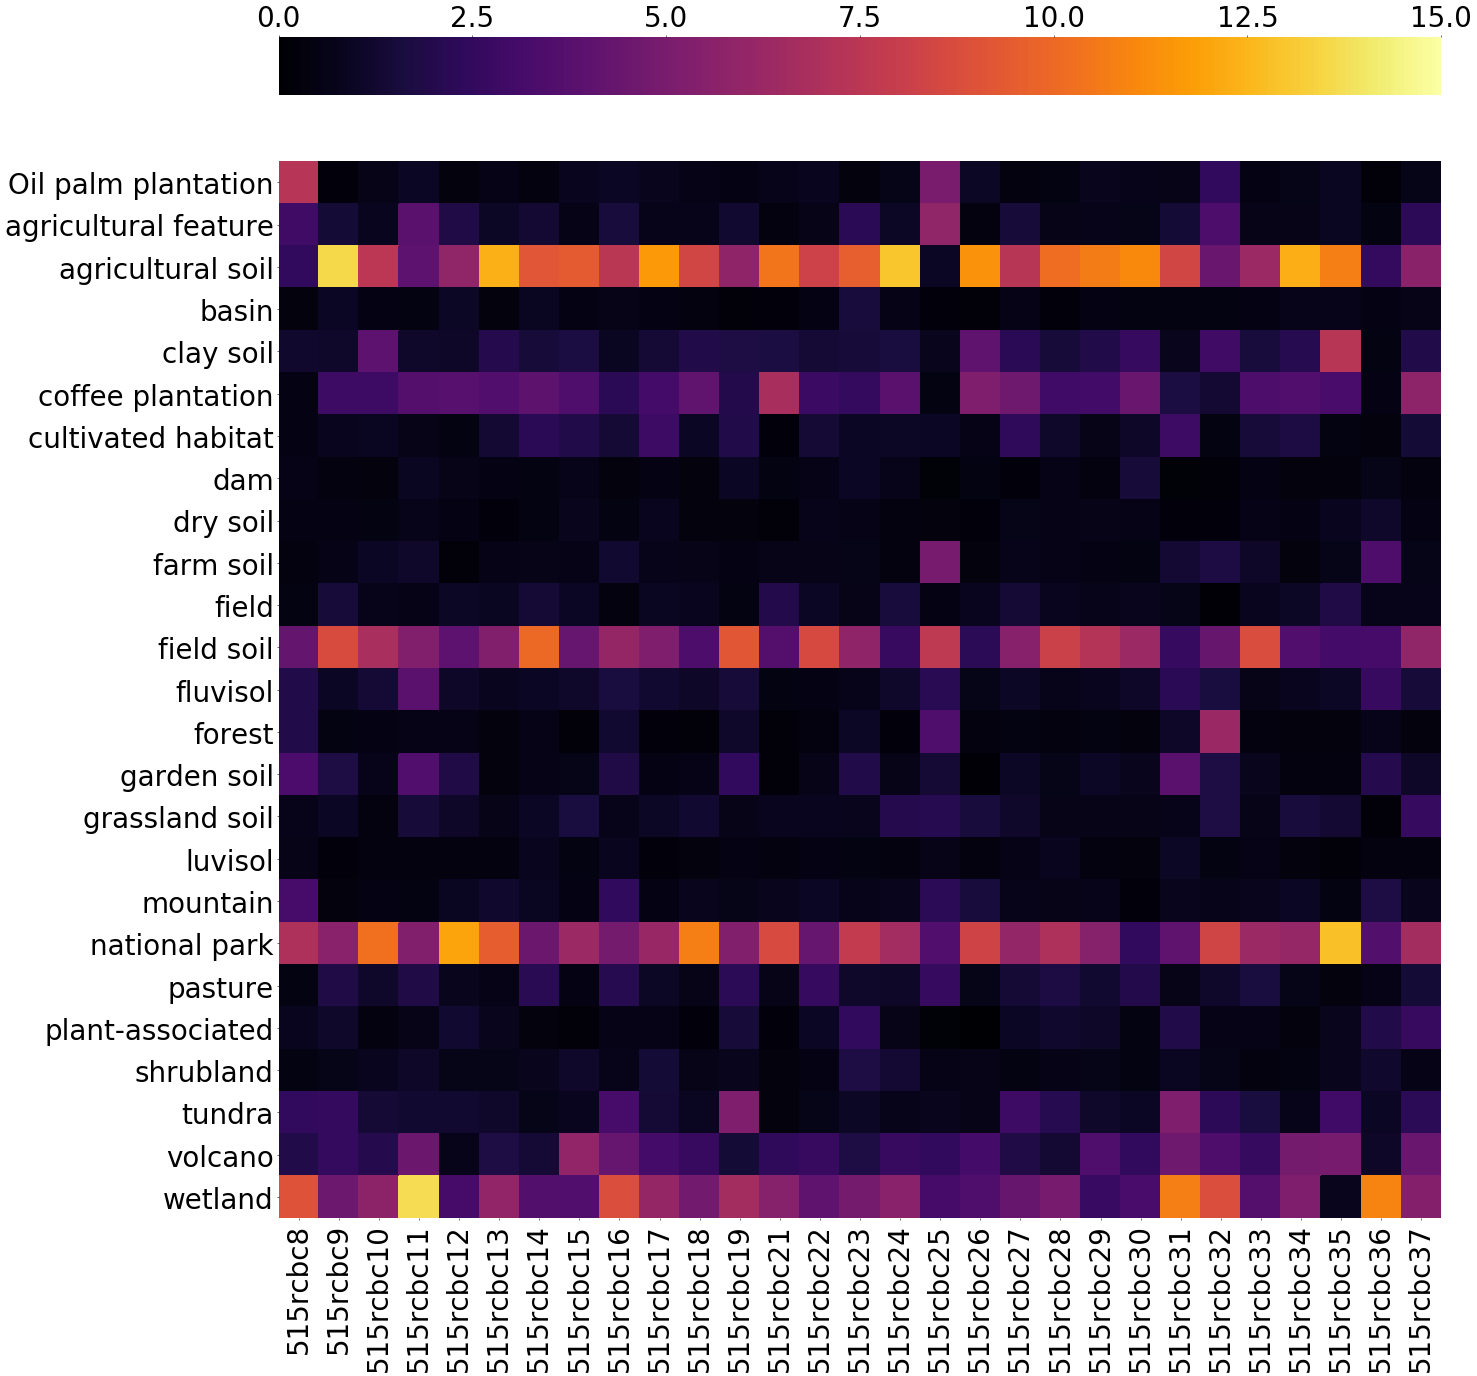
\includegraphics[width=\linewidth]{heatmap_perc.png}
	\caption{Heat map showing the percentage of each source in each sink, filtered to represent the top 25 sources. The "Unknown" column is not shown however, it represents a mean of 44\% of sources in each sink. As we can see there are 4 prominent sources in most sinks - agricultural soil, national park soil, wetland soil and field soil, which have a mean percentage of over 5\%.}
	\label{fig:Sourcetracker_heatmap}
\end{figure}
%
% DISCUSSION
%

\section{Discussion}
The results of the first steps in the computational pipeline show that the approach based on OTU picking does not provide the most accurate results. For instance, the SILVA database currently contains 177222 sequences, which means that our study, while being rather small, covered almost 10\% of the database. Thompson et al.\cite{Thompson2017} report that a study they performed using just under 100 samples from different biomes covered  47\% of the SILVA database. Low coverage of even the most up-to-date databases such as SILVA combined with the diminishing property of the OTU picking process creates the need for more accurate methods of sequence assessment, such as Deblur\cite{Amir}. 
\par
As we can see from the results of alpha and beta diversity analysis, our samples form a uniform collection, with samples \textit{515rcbc12}, \textit{515rcbc20} and \textit{515rcbc36} forming an array of aberrations. And while the first two were expected outliers due to the altered condition they were collected in, sample \textit{515rcbc36} is an unpredicted outlier, because it had an identical metadata to other samples, which suggests that the sample was contaminated. Further analysis is required to prove this hypothesis however, if the samples were to be included in the EMP it is preferential the three outliers.
\par
The hypothesis of the 27 samples forming a uniform sample is supported by the taxonomic assessment of the samples. While most samples show a similar composition, the three outlier samples mentioned above have atypical proportions of various phyla, confirming them as outliers.
\par
Overall, taxonomy of the dataset as a whole is quite typical and is similar to the results of park soil taxonomy analysis performed by Zhalnina et al.\cite{Zhalnina2014}. Their research was performed on samples of soil from a park in United Kingdom however, with a higher focus on taxonomy. Similarity of our results further strengthens the hypothesis that our dataset, with the exception of the outliers is a good representative of urban park soil and is valid enough to be included in the EMP.
\par
Sourcetracker analysis produced quite intriguing results.  Since our samples were collected in Gordon Square in Central London, an anthropomorphic biome, high relatedness to agricultural soil and field soil was expected. The unifying feature of such environments is a heavy use of fertilizers, which leads to development of specific ecosystems. This confirms that our samples can be safely compared with larger datasets such as the EMP. However, the peculiarities such as high relatedness to the wetland biome require further investigation.
\par
The absence of correlation within out dataset happened for a variety of reasons. Firstly, the quality of kits used to obtain the metadata was subpar and such measurements should have been performed using appropriate scientific equipment. Secondly, the uniformity and tight clustering of the samples hinders any attempts to discover correlations between the genetic data and metadata. A purposeful diversification of samples is paramount in such experiments, for example introducing difference in location, season or other conditions. Since 27 of the samples were collected from the same location at the same time, there is very low variance in the data and the few outliers can only provide anecdotal evidence.
\par
However, it must be noted that the samples would be a good addition to the existing microbiome databases such as EMP, since it was confirmed by multiple tests that the majority of the dataset, with the exception of 3 outlier samples is rather uniform and is representative of soil in urban biome. Despite that, the stand-alone scientific value of the dataset is minuscule, due to absence of correlation most of the parameters within the dataset. In order to obtain data that can provide researchers with statistically significant results, the diversity of samples and methods of metadata collection must be improved, and use of reference-free sequence analysis techniques is preferential.
\par
In conclusion it must be said that the experiment described in this paper can be well epitomized by the proverb "a chain is only as strong as its weakest link". While the methods of \textit{in silico} analysis were on a high level and extraction of the DNA from soil samples was performed without major complications the inferior results obtained in some crucial steps led to this research not providing scientifically valuable outcome. 

\bibliography{/home/ilya/Documents/Citations/3301.bib}
\end{document}